\subsection{逆紧作用于拓扑空间的群}

定义 1 设 G 是连续作用在拓扑空间 X 上的一个拓扑群。如果映射

\[
\theta : (s, x) \rightarrow (x, s. x) \text{ 从 } \mathbf{G} \times \mathbf{X} \text{ 到 } \mathbf{X} \times \mathbf{X}
\]

是逆紧的（第一章 § 10 第 1 目定义 1），就称 G 逆紧作用在 X 上。

设 \(\Gamma \subset \mathbf{G} \times \mathbf{X} \times \mathbf{X}\) 是映射 \(\rho: (s, x) \to s.x\) 的图。由于 \(\rho\) 连续，映射 \(\sigma: (s, x) \to (s, x, s.x)\) 是 \(\mathbf{G} \times \mathbf{X}\) 到 \(\Gamma\) 上的一个同胚，且复合映射

\[
\mathbf {G} \times \mathbf {X} \xrightarrow {\sigma} \Gamma \xrightarrow {\mathrm{pr} _ {2 3}} \mathbf {X} \times \mathbf {X}
\]

就是 \(\theta\)。因此定义 1 等价于说 \(\operatorname{pr}_{23}\) 在 \(\Gamma\) 上的限制是 \(\Gamma\) 到 \(\mathbf{X} \times \mathbf{X}\) 中的一个逆紧映射。

第一章 § 10 第 2 目定理 1 表明，G 逆紧作用在 X 上，当且仅当下列条件满足：

对每个由超滤子 F 过滤的集 A，以及每个映射

\[
\alpha \rightarrow (s _ {\alpha}, x _ {\alpha})
\]

（A 到 \(\mathbf{G} \times \mathbf{X}\) 中的），如果映射 \(\alpha \to (s_{\alpha}.x_{\alpha}, x_{\alpha})\) 有一个极限 \((b, a)\)（关于 \(\mathfrak{F}\) 的），则 \(\alpha \to s_{\alpha}\) 有一个极限 \(t \in \mathbf{G}\)（关于 \(\mathfrak{F}\) 的），使得 \(t.a = b\)。

例。1) 设 H 是拓扑群 G 的一个闭子群。若 G 逆紧作用在 X 上，则 H 也逆紧作用在 X 上，因为 H × X 在 G × X 中是闭的（第一章 § 10 第 1 目命题 5 推论 1）。例如若取 X = G，G 通过左平移作用在自身上，则映射 G × X → X × X 是一个同胚，因而是逆紧的；于是 H 通过左平移逆紧作用在 G 上。

\begin{enumerate}
\def\labelenumi{\arabic{enumi})}
\setcounter{enumi}{1}
\tightlist
\item
  若 G 逆紧作用在 X 上，则它逆紧作用在 X 的每个子空间 \(X'\)（它是 X 的点的轨道的并）上（换言之，\(X'\) 关于由 G 定义的等价关系是饱和的）。因为 \(X' \times X'\) 在 \(G \times X\) 中的原像是 \(G \times X'\)，且我们可以应用第一章 § 10 第 1 目命题 3。
\end{enumerate}

命题 1 设 G 是连续作用在拓扑空间 X 上的一个拓扑群，K 是 G 的一个拟紧子集。则映射 \(\rho: (s, x) \to s.x\)（\(K \times X\) 到 \(X\) 中的）是逆紧的。

\(\rho\) 分解为 \(\mathbf{K} \times \mathbf{X} \to \mathbf{K} \times \mathbf{X} \xrightarrow{\mathrm{pr}_2} \mathbf{X}\)，其中 \(\alpha(s, x) = (s, s.x)\)。\(\alpha\) 是一个同胚，因为 \(\alpha^{-1}: (s, y) \to (s, s^{-1}.y)\) 连续。由于 \(\mathbf{K}\) 是拟紧的，\(\mathrm{pr}_2\) 是逆紧的（第一章 § 10 第 2 目定理 1 推论 5）；因而 \(\rho\) 是逆紧的（第一章 § 10 第 1 目命题 5）。

推论 1 若 A 是 X 的一个闭（相应地紧）子集，则 K.A 在 X 中是闭的（相应地，若 X 是 Hausdorff 的，则是紧的）。

关于闭集的断言由命题 1 以及逆紧映射是闭映射这一事实（第一章 § 10 第 1 目命题 1）得出。关于紧集的断言是显然的。

\pandocbounded{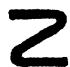
\includegraphics[keepaspectratio]{images/part002_62417fce.jpg}}

应当注意，若 L 是 X 的一个紧子集，F 是 G 的一个闭子集，则 F. L 在 X 中未必是闭的（§ 2 习题 29；参看第 5 目命题 12 的推论）。

推论 2 若 K 是拓扑群 G 的一个拟紧子群，则等价关系 \(x^{-1}y \in K\) 是闭的，且典范映射 \(\varphi: G \to G/K\) 是逆紧的。

第一个断言由推论 1 应用于通过右平移作用在自身上的 G 得出，第二个断言则由第一章 § 10 第 2 目定理 1 得出。

推论 3 设 K 是拓扑群 G 的一个拟紧正规子群，\(\varphi\) 是典范映射 G → G/K。则对 G 的每个闭子群 A，A/A∩K 到 \(\varphi(A)\) 上的典范双射是拓扑群的一个同构。

由于 \(x^{-1}y \in K\) 是一个闭等价关系（推论 2），本推论由第一章 § 5 第 2 目命题 4 得出。

命题 2 设 K 是连续作用在 Hausdorff 空间 X 上的一个紧群。则：

\begin{enumerate}
\def\labelenumi{\alph{enumi})}
\item
  K 逆紧作用在 X 上。
\item
  映射 \((s, x) \to s.x\)（\(\mathbf{K} \times \mathbf{X}\) 到 \(\mathbf{X}\) 中的）是逆紧的。
\item
  X 到 X/K 上的典范映射是逆紧的。
\item
  是命题 1 的推论。至于 a)，由于 K 是紧的，\(\operatorname{pr}_{2}:(s,x)\to x\) 是逆紧的（第一章 § 10 第 2 目定理 1 推论 5）；因而，由于 X 是 Hausdorff 的，\((s,x)\to(x,s.x)\) 是逆紧的（第一章 § 10 第 1 目命题 5 推论 3）。剩下证明 c)。依命题 1 的推论 1，典范映射 \(\varphi:X\to X/K\) 是闭的。若 Z 是任一拓扑空间且让 K 平凡作用在 Z 上，则 K 连续作用在 \(X\times Z\) 上，因而典范映射 \(X\times Z\to(X\times Z)/K\) 是闭的。但 \((X\times Z)/K\) 可以典范地等同于 \((X/K)\times Z\)（§ 2 第 4 目引理 2 及第一章 § 5 第 3 目命题 8 的推论）；因而典范映射 \(X\times Z\to(X\times Z)/K\) 可以等同于 \(\varphi\times1\)，且由于它对所有 Z 是闭的，可知 \(\varphi\) 是逆紧的。
\end{enumerate}

推论 1 在命题 2 的假设下，X 是紧的（相应地局部紧的），当且仅当 X/K 是紧的（相应地局部紧的）。

这由典范映射 \(X \rightarrow X/K\) 是逆紧的这一事实得出，依据第一章 § 10 第 4 目命题 9。

推论 2 设 G 是一个 Hausdorff 拓扑群，K 是 G 的一个紧子群。则 G 是紧的（相应地局部紧的），当且仅当 G/K 是紧的（相应地局部紧的）。

对通过右平移作用在 G 上的 K 应用推论 1。
% semantic-fragments: legacy-input-seam
\relax{}
